\documentclass[11  pt]{article} 
\usepackage[lmargin=1in,rmargin=1.75in,bmargin=1in,tmargin=1in]{geometry}  


% For hyperlinking everything
\usepackage{hyperref}
\hypersetup{
	colorlinks=true, %set true if you want colored links
	linktoc=all,     %set to all if you want both sections and subsections linked
	linkcolor=blue,  %choose some color if you want links to stand out
}


\usepackage[latin1]{inputenc}
\usepackage{amsmath}
\usepackage{mathrsfs}  
\usepackage{amsfonts}
\usepackage{amssymb}
\usepackage{graphicx}
\usepackage{subfig}
\usepackage{caption}
\usepackage{algorithm}
%\usepackage{algcompatible}
%\usepackage{algorithmicx}
\usepackage{algpseudocode}

\usepackage{titlesec}
\titleformat{\section}{\fontfamily{lmss}\fontsize{14}{15}\bfseries}{\thesection}{1em}{}
\titleformat{\subsection}{\fontfamily{lmss}\fontsize{12}{15}\bfseries}{\thesubsection}{1em}{}




\usepackage{amsthm}

\newtheoremstyle{noit}
{10pt}% <Space above>
{10pt}% <Space below>
{}% <Body font>
{}% <Indent amount>
{\bfseries}% <Theorem head font>
{.}% <Punctuation after theorem head>
{.5em}% <Space after theorem headi>
{}% <Theorem head spec (can be left empty, meaning `normal')>

\newtheoremstyle{example}
{10pt}% <Space above>
{10pt}% <Space below>
{}% <Body font>
{20pt}% <Indent amount>
{\bfseries}% <Theorem head font>
{.}% <Punctuation after theorem head>
{.5em}% <Space after theorem headi>
{}% <Theorem head spec (can be left empty, meaning `normal')>


\newtheoremstyle{indented}{20pt}{20pt}{\addtolength{\leftskip}{2.5em}}{}{\bfseries}{.}{.5em}{}


\newtheorem{theorem}{Theorem}
\numberwithin{theorem}{section}
\newtheorem{lemma}[theorem]{Lemma}
\newtheorem{corollary}[theorem]{Corollary}
\newtheorem{observation}{Observation}
%\numberwithin{observation}{section}
%\numberwithin{definition}{section}
\newtheorem{conjecture}{Conjecture}
\newtheorem{Qu}{Question}
\newcommand{\QU}{\begin{Qu}\normalfont}

\theoremstyle{noit}
\newtheorem{fact}{Fact}
\newtheorem{definition}{Definition}

\theoremstyle{indented}
\newtheorem{example}{Example}

\theoremstyle{indented}
\newtheorem{problem}{Problem}


%\newenvironment{proof}{\noindent{\bf Proof:} \hspace*{1em}}{
%    \hspace*{\fill} $\Box$ }
%\newenvironment{proof_of}[1]{\noindent {\bf Proof of #1:}
%    \hspace*{1em} }{\hspace*{\fill} $\Box$ }
%\newenvironment{proof_claim}{\begin{quotation} \noindent}{
%    \hspace*{\fill} $\diamond$ \end{quotation}}
\newcommand{\vs}[1]{\vspace{#1}}

\newcommand{\lecture}[2]{
 \noindent
\begin{center}
	\framebox{
		\vbox{
			\hbox to 5.78in { {\bf CSCE 411: Design and Analysis of Algorithms} \hfill  }
			\vspace{2mm}
			\hbox to 5.78in { {\Large \hfill Lecture #1\hfill} }
			\vspace{2mm}
			\hbox to 5.78in { {\it Date: #2 \hfill Lecturer: Nate Veldt} }
		}
	}
\end{center}
\vspace*{4mm}
}


\newcommand{\hw}[2]{
	\noindent
	\begin{center}
		\framebox{
			\vbox{
				\hbox to 5.78in { {\bf CSCE 411: Design and Analysis of Algorithms} \hfill  }
				\vspace{2mm}
				\hbox to 5.78in { {\Large \hfill Homework #1\hfill} }
				\vspace{2mm}
				\hbox to 5.78in { {\it Due date: #2 \hfil} }
			}
		}
	\end{center}
	\vspace*{4mm}
}



\newcommand{\under}[1]{\underline{\hspace{#1}}}
\setlength{\parindent}{0em}

%\usepackage[tagged]{accessibility}

% Graph terms
\newcommand{\vol}{\textbf{vol}}
\newcommand{\cut}{\textbf{cut}}


% Matrices
\newcommand{\mA}{\textbf{A}}
\newcommand{\mB}{\textbf{B}}

% vectors
\newcommand{\ve}{\textbf{e}}
\newcommand{\vx}{\textbf{x}}


% Other
\newcommand{\calN}{\mathcal{N}}

\usepackage{mathtools}
\DeclarePairedDelimiter\ceil{\lceil}{\rceil}
\DeclarePairedDelimiter\floor{\lfloor}{\rfloor}


\newcommand*{\aitem}{ \item[{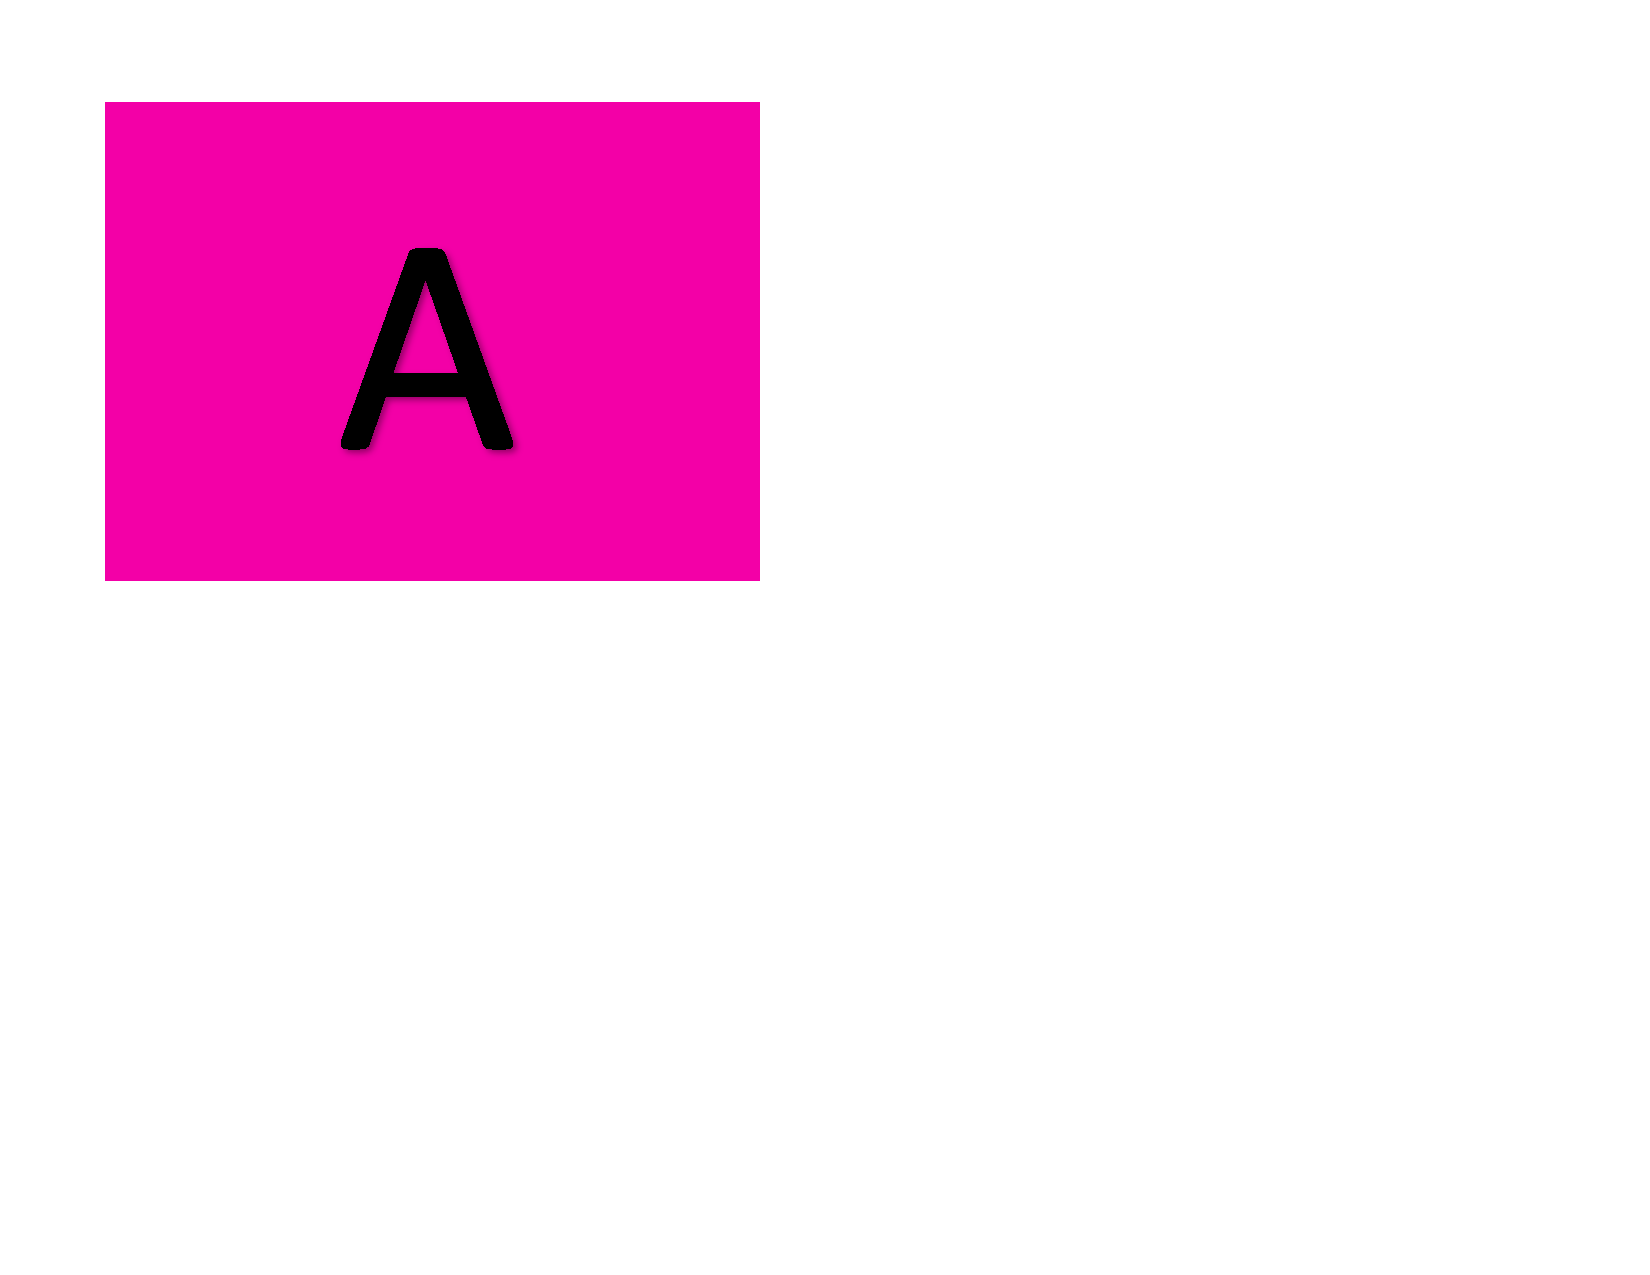
\includegraphics[width=0.8cm,height=0.5cm]{../../Lectures/figures/A}} ]  }
\newcommand*{\bitem}{ \item[{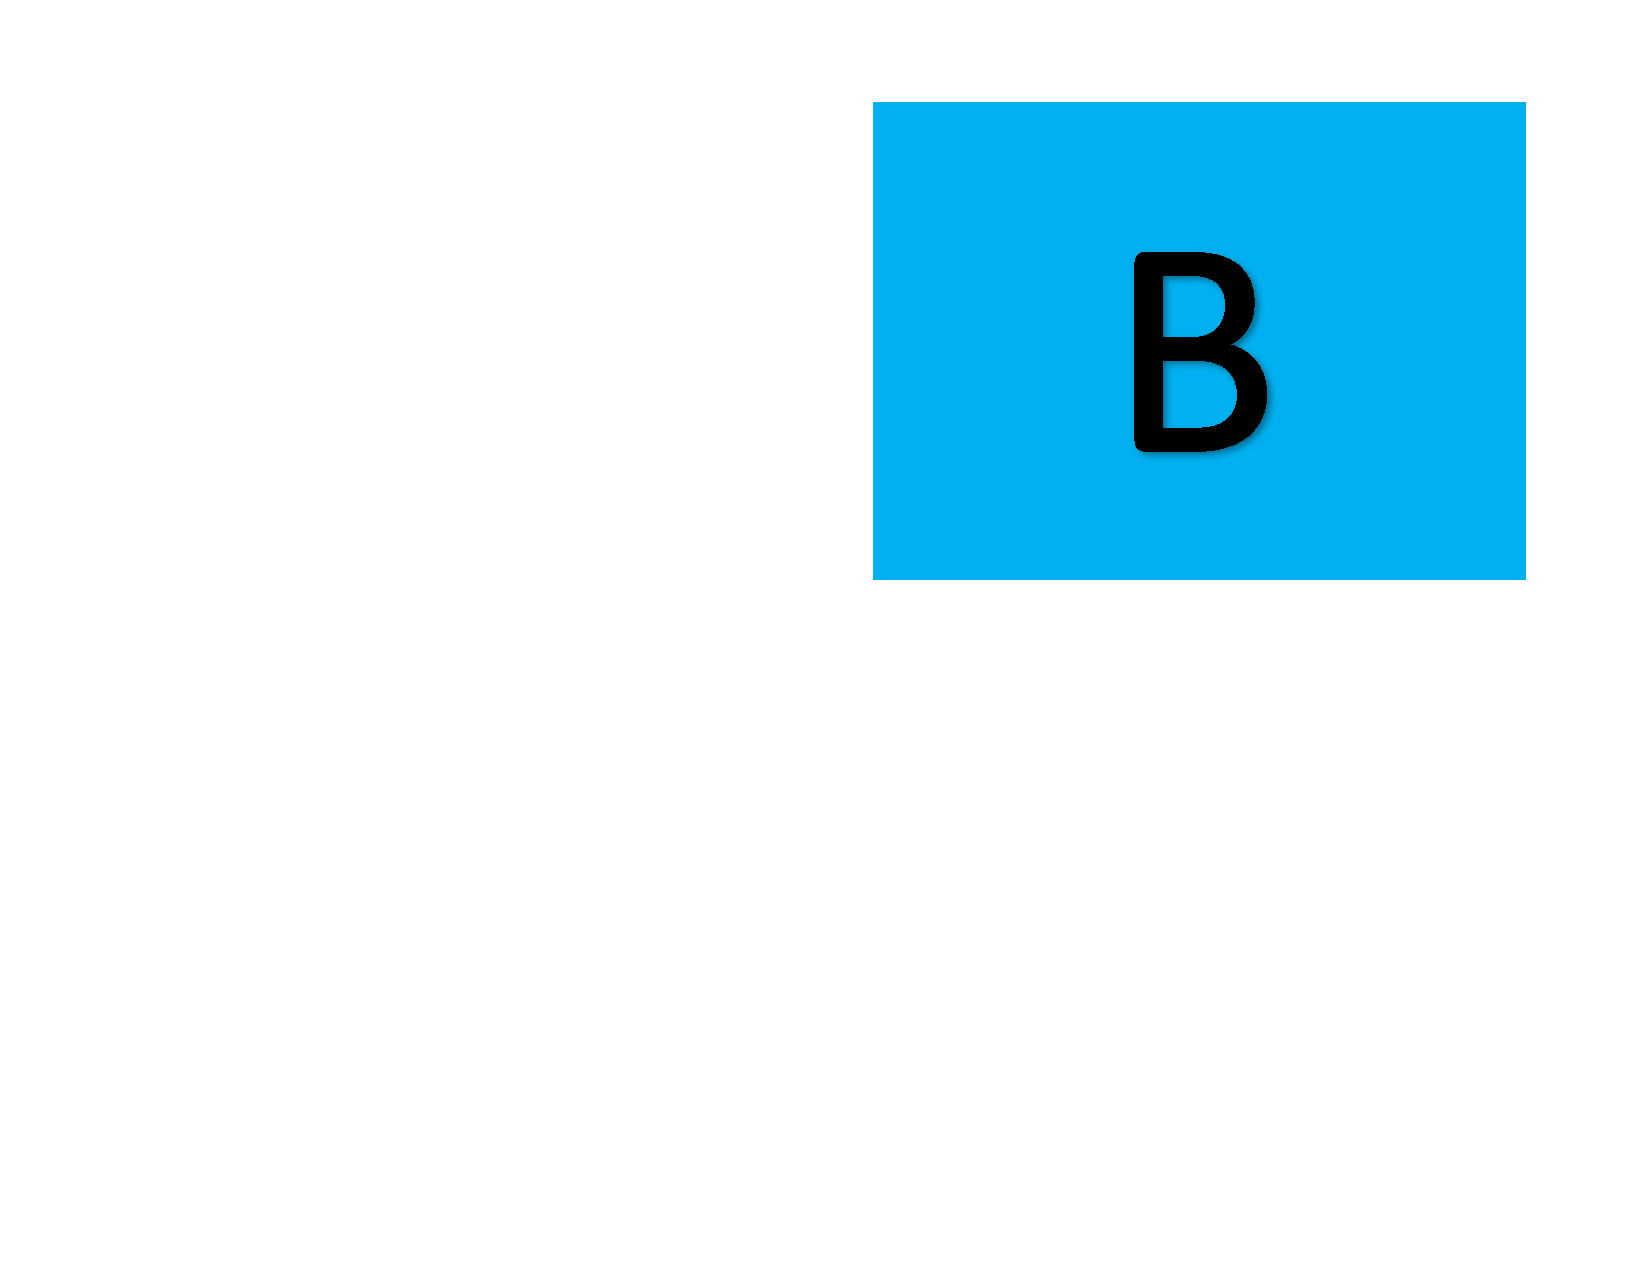
\includegraphics[width=0.8cm,height=0.5cm]{../../Lectures/figures/B}} ]  }
\newcommand*{\citem}{ \item[{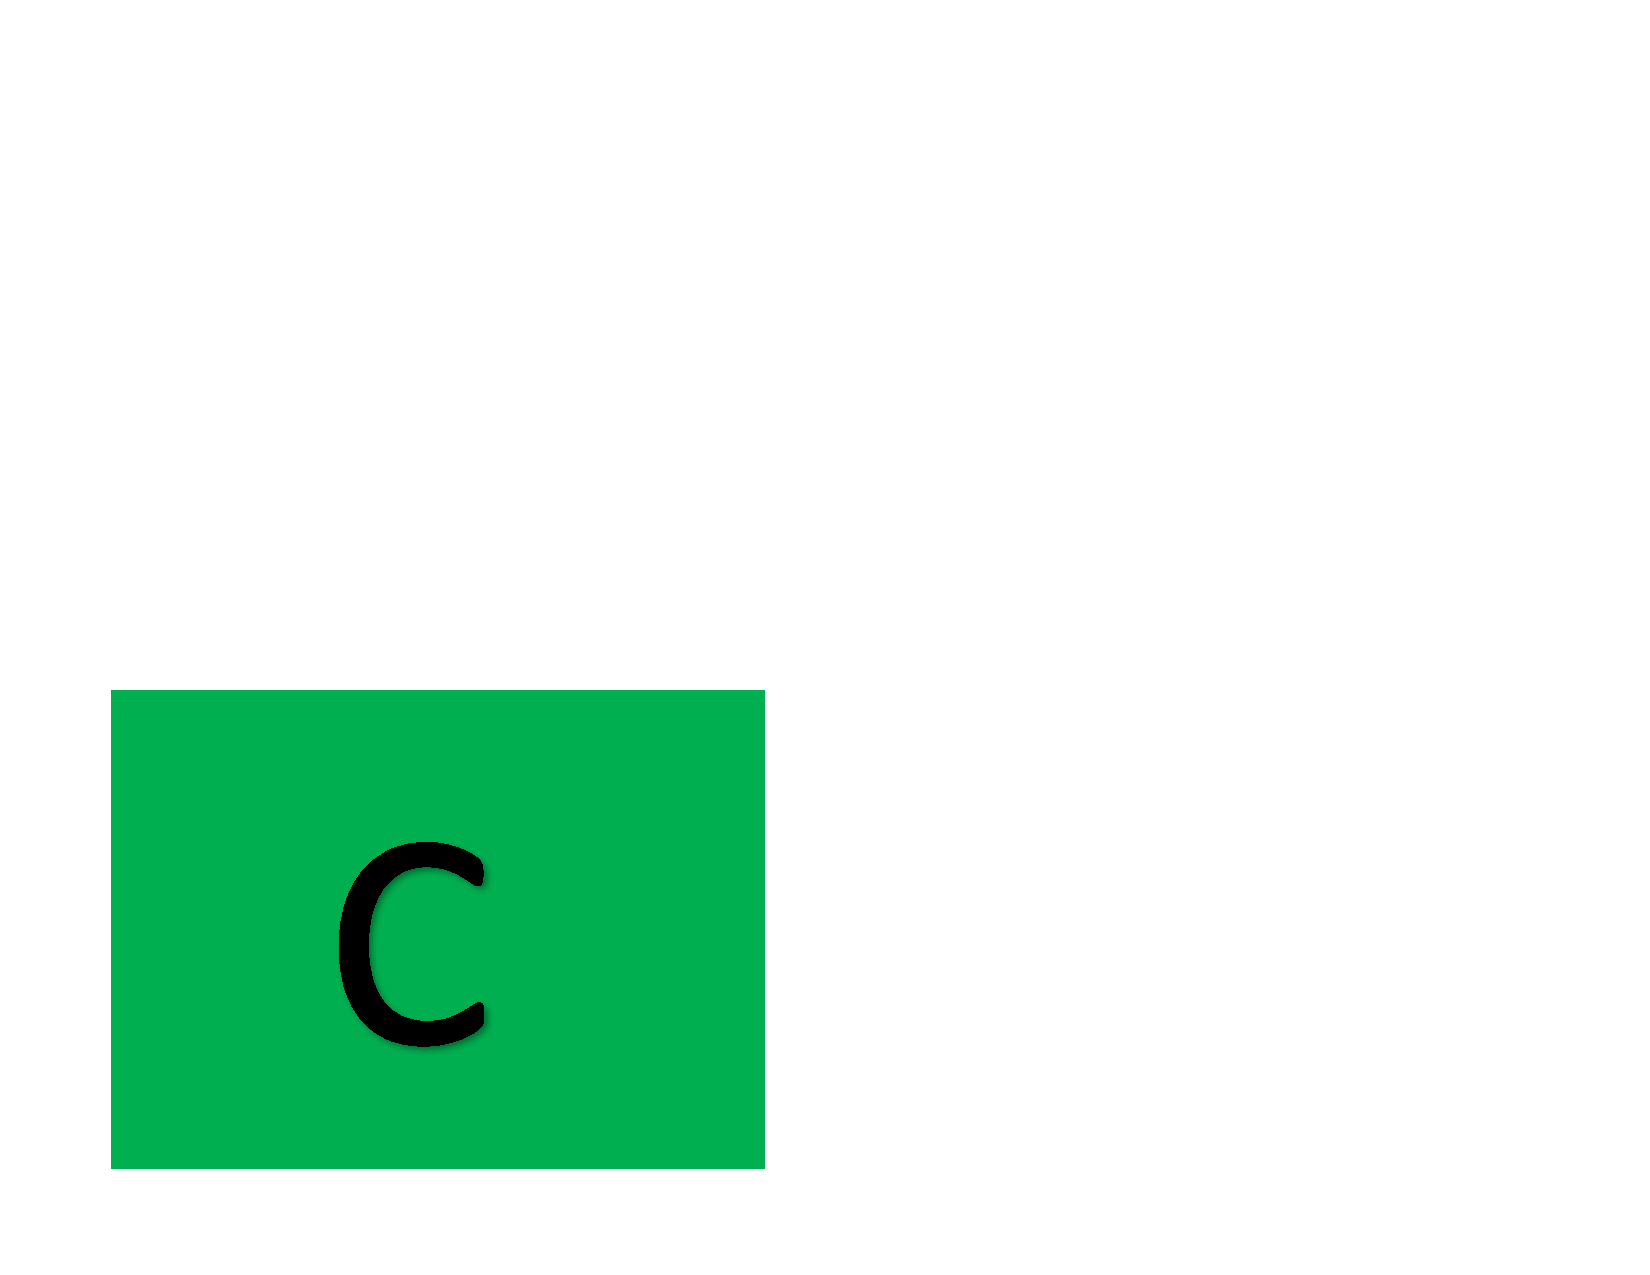
\includegraphics[width=0.8cm,height=0.5cm]{../../Lectures/figures/C}} ]  }
\newcommand*{\ditem}{ \item[{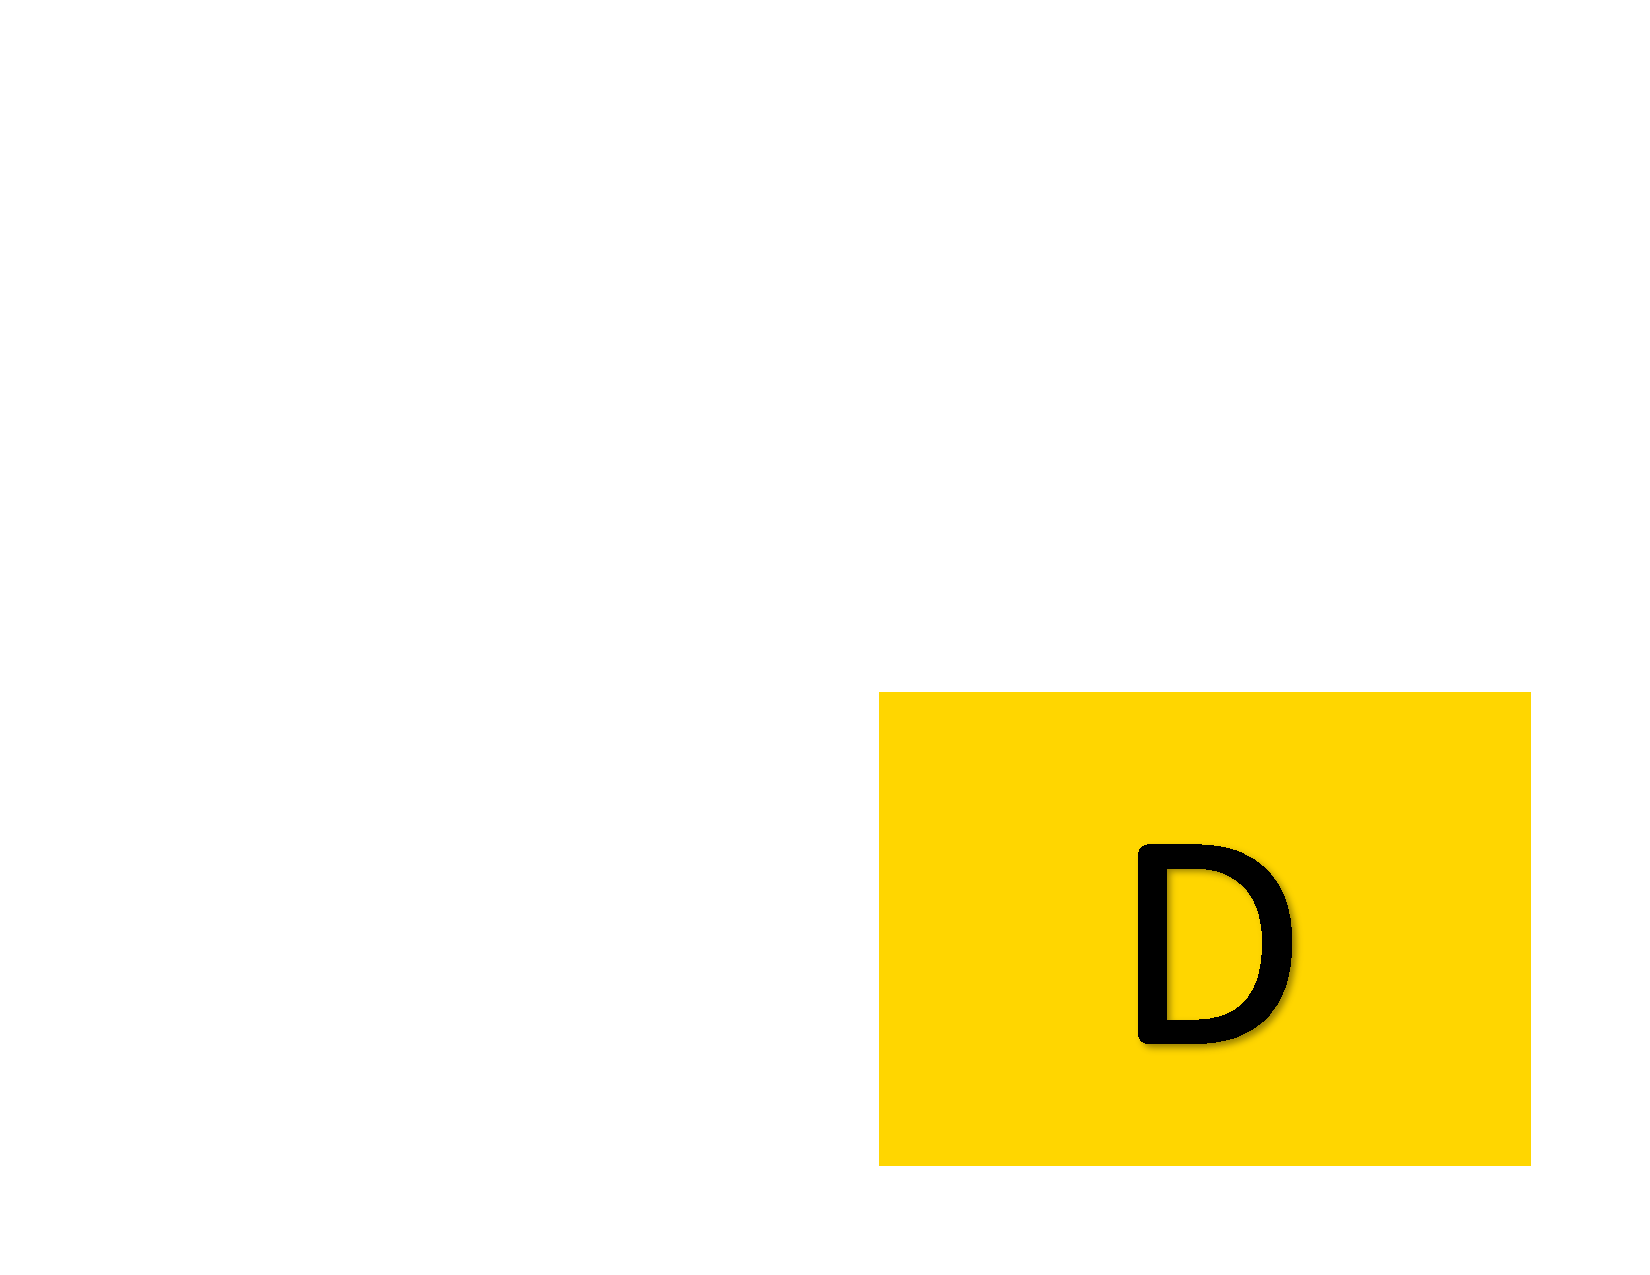
\includegraphics[width=0.8cm,height=0.5cm]{../../Lectures/figures/D}} ]  }
\newcommand*{\eitem}{ \item[{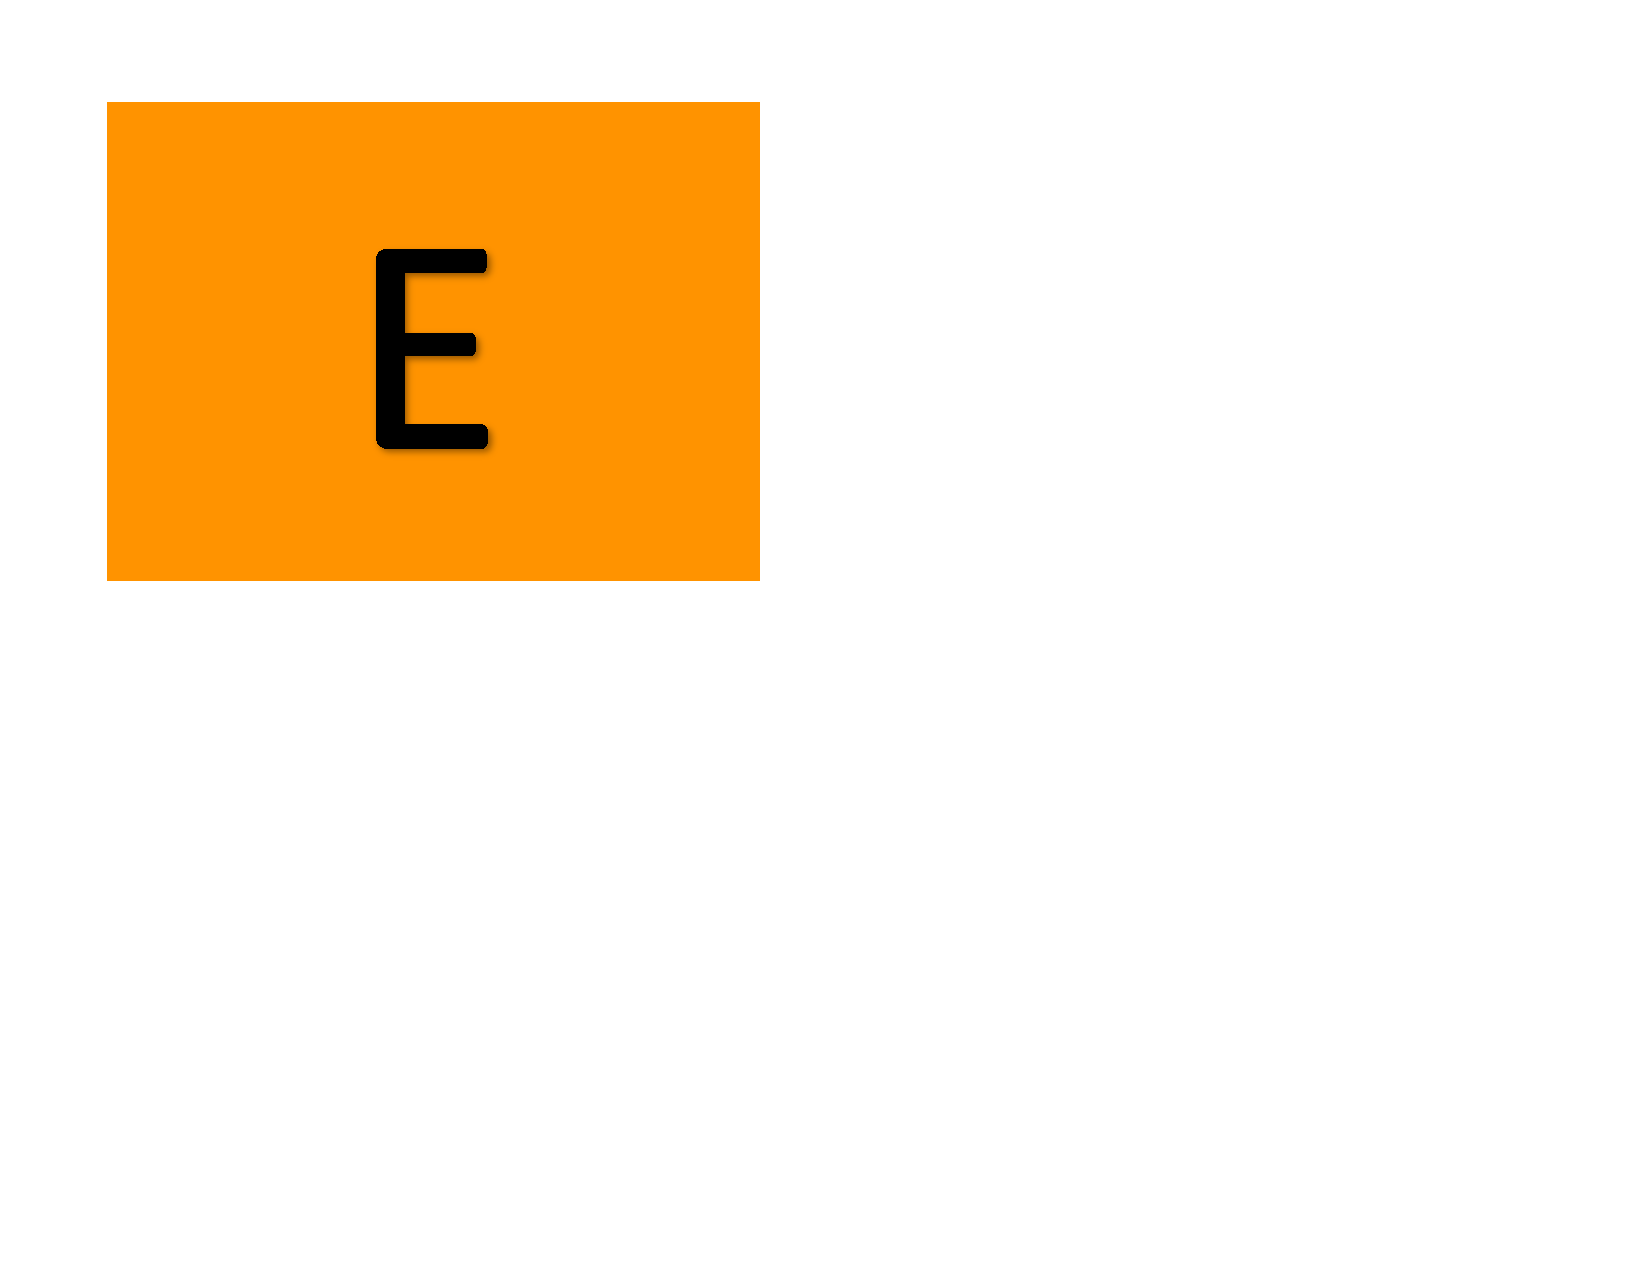
\includegraphics[width=0.8cm,height=0.5cm]{../../Lectures/figures/E}} ]  }
\newcommand*{\fitem}{ \item[{
\includegraphics[width=0.8cm,height=0.5cm]{../../Lectures/figures/F}} ]  }


\newcommand{\hide}[1]{\underline{\phantom{#1 #1}}}

\usepackage{setspace}

\onehalfspacing

\begin{document}
	
	\lecture{17-18: Maximum $s$-$t$ Flow}{Week 10}
	
	\paragraph{Course Logistics}
	\begin{itemize}
		\item Reading from Chapter 26 this week
		\item Homework 7 has been posted, due on Friday
		\item Test 2 next Thursday; Review next Tuesday
	\end{itemize}
	
	\section{The Maximum $s$-$t$ Flow Problem}
	
	\paragraph{Input to the Maximum $s$-$t$ Flow Problem}
	\begin{itemize}
		\item A weighted and directed graph $G = (V,E,w)$
		\item A source node $s$
		\item A sink node $t$
	\end{itemize}
	
	\textit{Goal}: Route as much ``flow'' through the graph from $s$ to $t$ as possible, such that:
	\begin{itemize}
		\item The flow on an edge is bounded by 
		\item The flow into a node (except for $s$ and $t$) is equal to 
		%the flow out of a node 
	\end{itemize}
	
	\begin{center}
		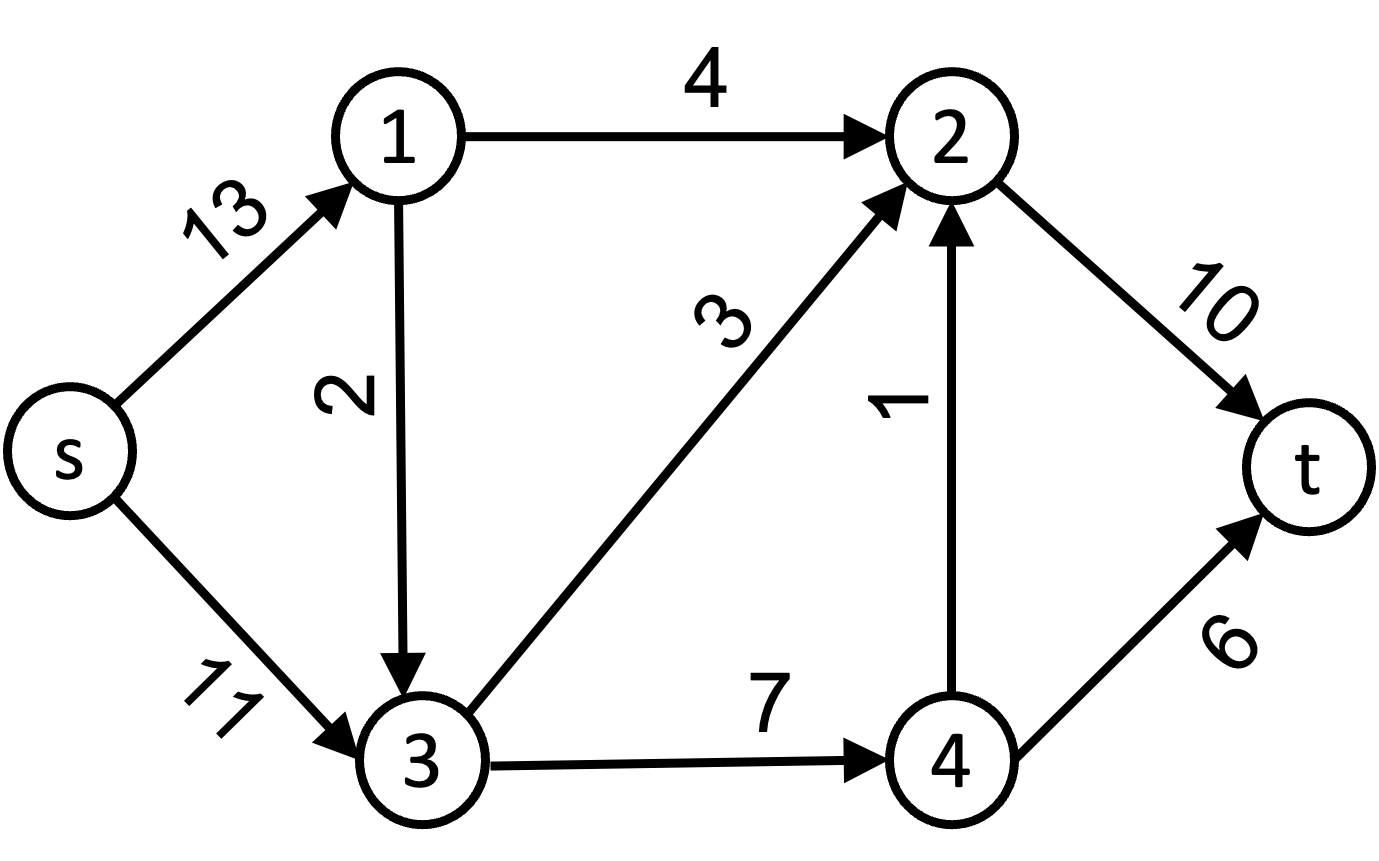
\includegraphics[width = .65\linewidth]{flow1.png} \\
	\end{center}
	
	One interpretation/application: transporting products/merchandise as efficiently as possible through a transportation network.
	
	
	\newpage
	
	\subsection{Defining $s$-$t$ flows more formally}
	Given a weighted graph $G = (V,E,w)$, each $(u,v) \in E$ has a weight or \emph{capacity} $w(u,v) = c(u,v)$. \\
	
	A \emph{flow} on $G$ is a function
	\begin{equation}
		f \colon E\rightarrow \mathbb{R}
	\end{equation}
	that satisfies two properties:
	\begin{enumerate}
		\item \textbf{Capacity constraints}: for each edge $(u,v) \in E$:\\ \\
%		$$f(u,v) \leq c(u,v)$$
		\item \textbf{Flow constraints}: for each node $v \notin \{s,t\}$ \\
%		$$\sum_{u \colon (u,v) \in E} f(u,v) = \sum_{j \colon (v,j) \in E} f(v,j)$$
	\end{enumerate}
	\vs{3cm}
	% picture
	
	The \emph{value} of a flow $f$ is given by
	\begin{equation}
		|f| =  \sum_{ j\colon (s,j) \in E} f(s,j) - \sum_{u \colon (u,s) \in E} f(u,s)  
	\end{equation}
	
	\textbf{Formal goal}: find the flow function $f^*$ with maximum value $|f^*|$.
	
	\vs{1cm}
	
	\begin{center}
		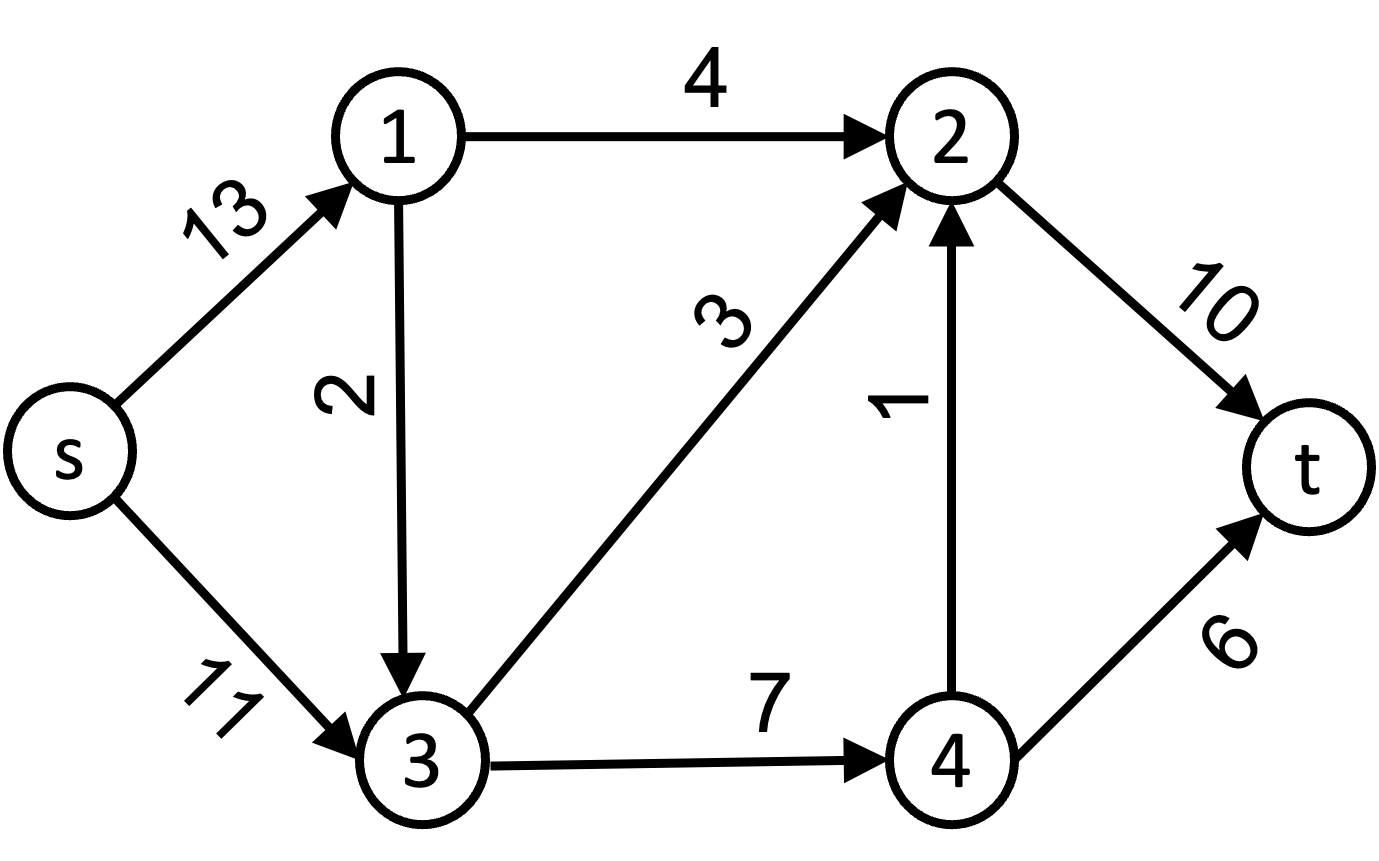
\includegraphics[width = .5\linewidth]{flow1.png} \\
	\end{center}
	\newpage
	
	\begin{Qu}
		What is the value of the flow $f$ below? 
		\begin{center}
			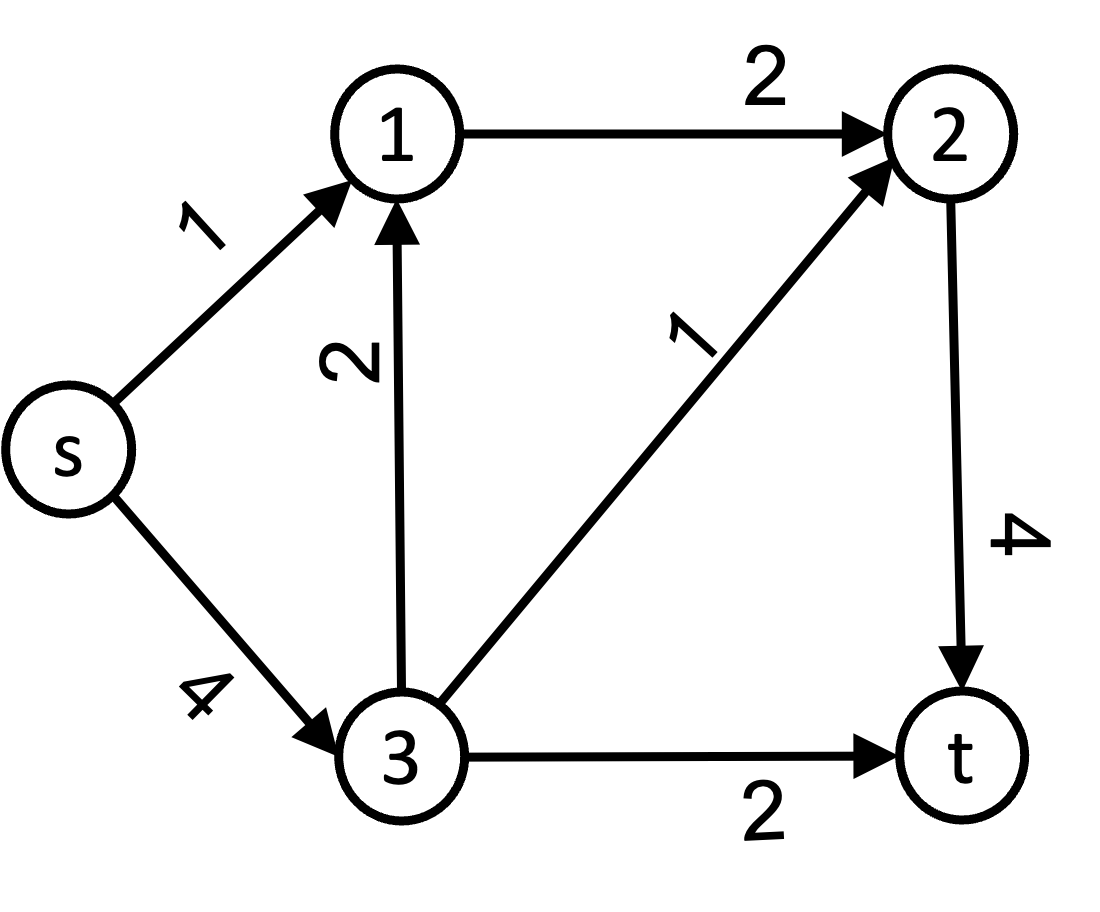
\includegraphics[width = .5\linewidth]{flow2.png} \\
		\end{center}
		\begin{itemize}
			\aitem 4
			\bitem 5
			\citem 10
			\ditem 15
		\end{itemize}
	\end{Qu}
	
	\vs{2cm}
	
	\begin{Qu}
		Is it a maximum flow?
		\begin{itemize}
			\aitem Yes it is
			\bitem No it is not
			\citem It depends
		\end{itemize}
	\end{Qu}
	
	\newpage
	
	\subsection{The minimum $s$-$t$ cut problem}
	The minimum $s$-$t$ cut problem takes the same type of input as the maximum $s$-$t$ flow: a weighted directed graph $G = (V,E,w)$ with $s$ and $t$ nodes.\\
	
	An \emph{$s$-$t$ cut} set is a set of nodes $S \subseteq V$ such that \\ %$s \in S$ and $t \in V - S$. \\
	
	The \emph{value} of the cut is the weight of edges that cross from $S$ to $V- S$. Formally:\\

	\vs{4cm}
	
	What is the cut value below, where $S$ is the set of gray nodes? \\
	
	\begin{center}
		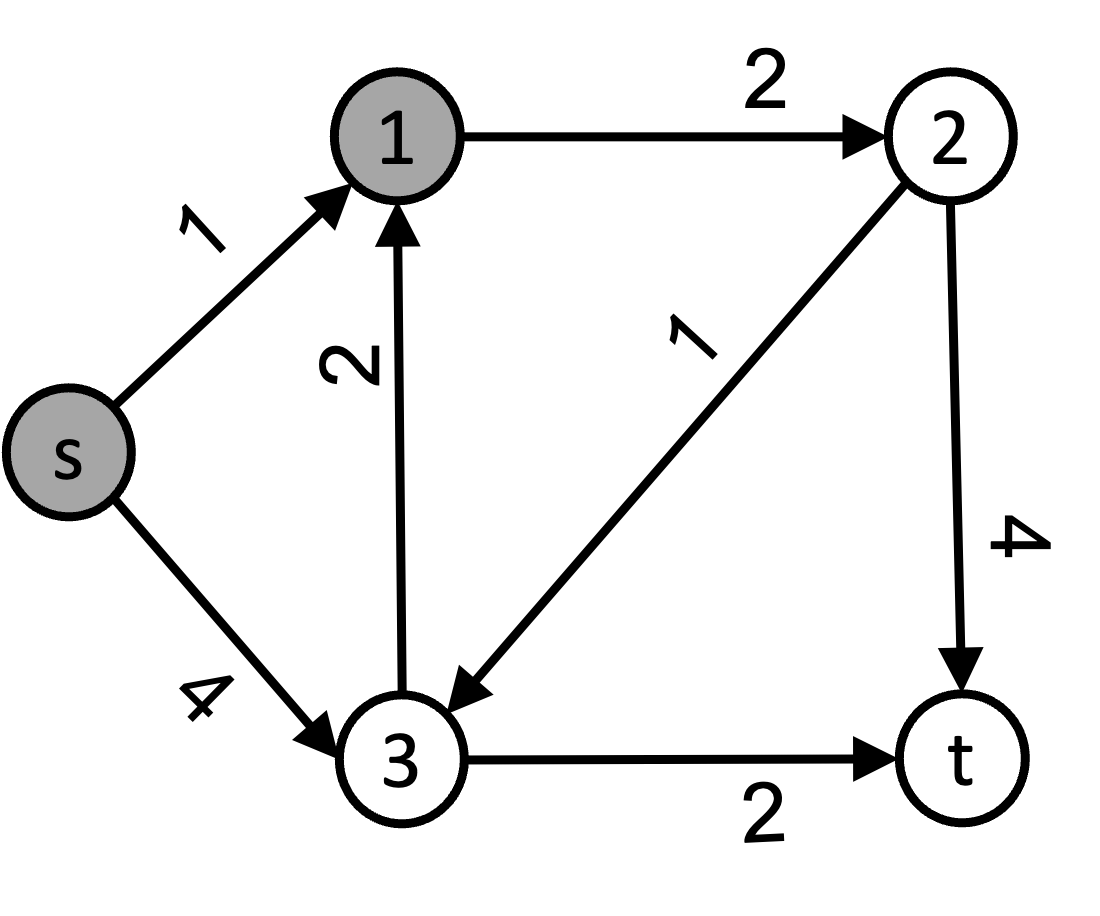
\includegraphics[width = .5\linewidth]{cut1.png} \\
	\end{center}
	
		\begin{Qu}
		What is the value of the flow $f$ below? 
		\begin{center}
			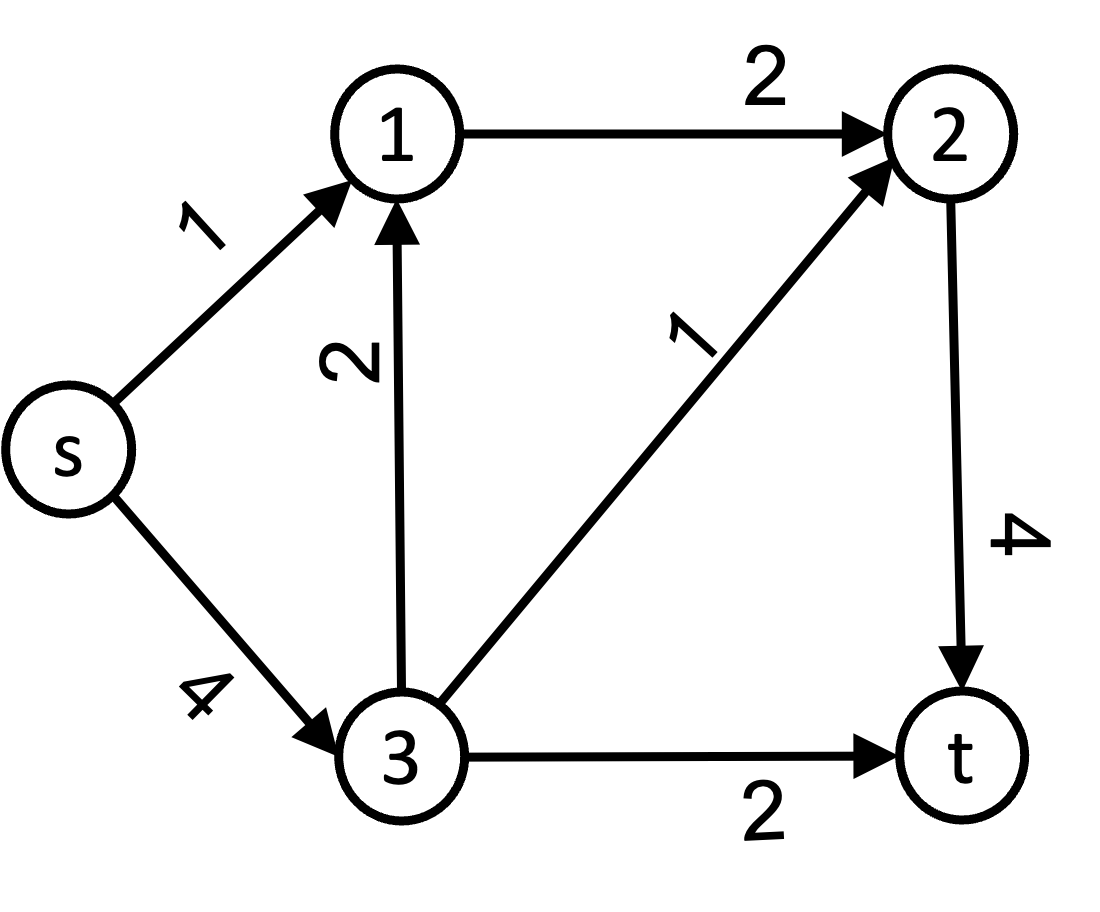
\includegraphics[width = .5\linewidth]{flow2.png} \\
		\end{center}
		\begin{itemize}
			\aitem 1
			\bitem 2
			\citem 6
			\ditem 8
		\end{itemize}
	\end{Qu}
	
	\newpage
	
	\subsection{Relating cuts and flows}
	
	
	\begin{lemma}
		Let $G = (V,E,w)$ be a weighted directed graph. Let $S \subseteq V$ be any set with $S$ be an $s$-$t$ cut set, and let $f$ be a flow. Then

	\end{lemma}
	
	
	\newpage
	
	Consider the following graph. Find the optimal $s$-$t$ flow value and then prove that it is optimal.
	\begin{center}
		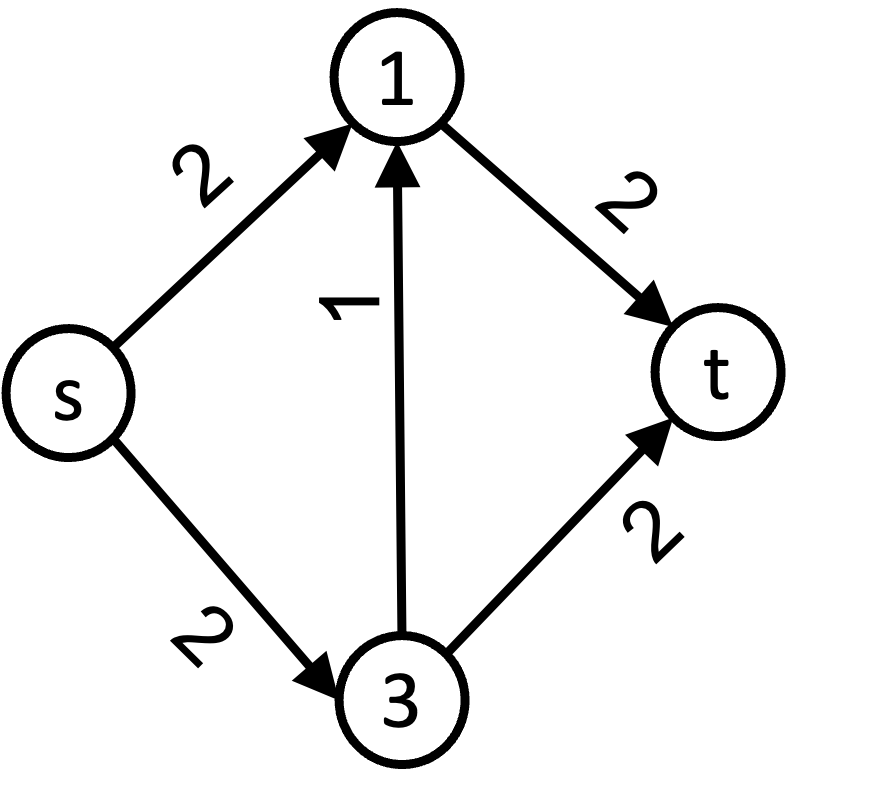
\includegraphics[width = .5\linewidth]{flow3.png} \\
	\end{center}
	
	
	\newpage
		\section{Finding maximum $s$-$t$ flow}
	
	\paragraph{First idea.} Repeatedly find paths from $s$ to $t$, and keep adding flow until there are no more $s$-$t$ paths. \\
	
	
	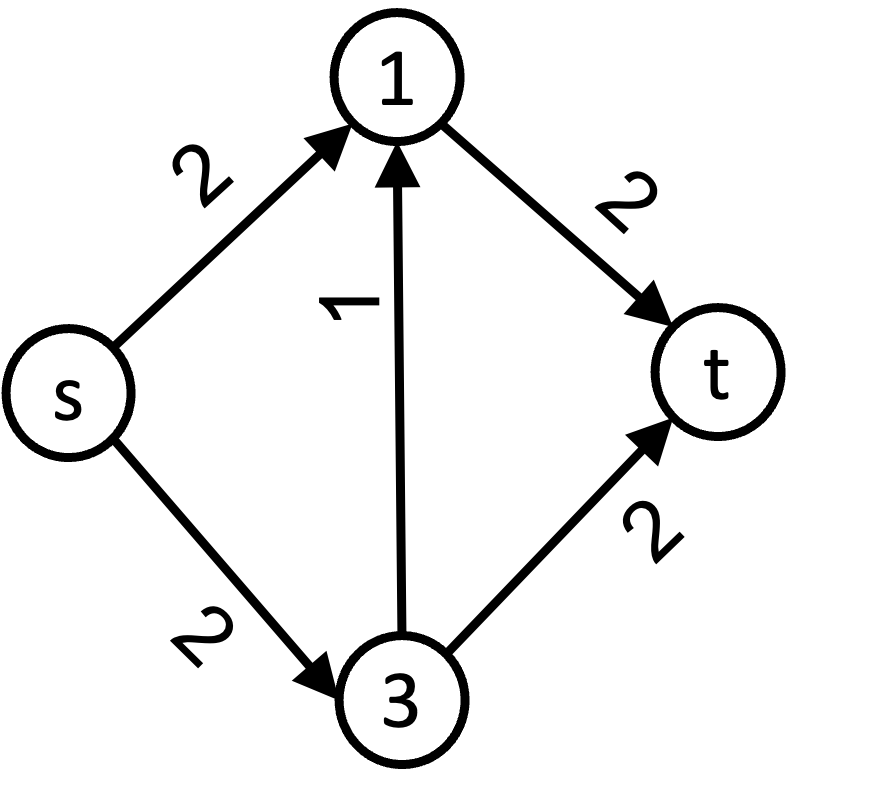
\includegraphics[width = .4\linewidth]{flow3.png} \hspace{2cm} 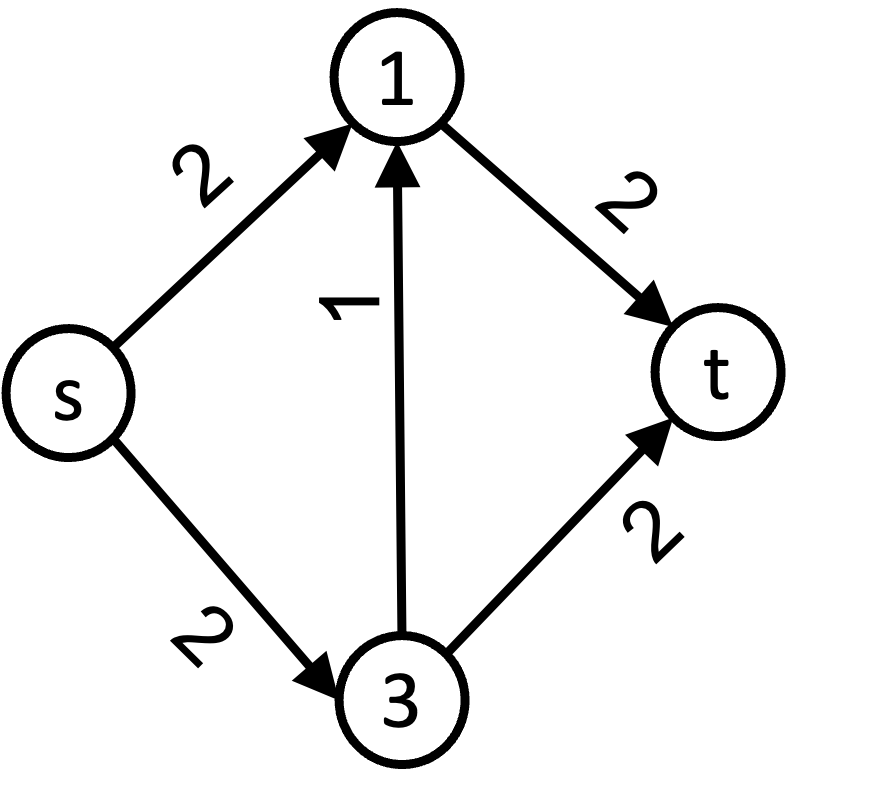
\includegraphics[width = .4\linewidth]{flow3.png} 
	
	How do we correct this? Let's try to keep track of flow that we could ``undo''.
	
	\subsection{The Residual Graph}
	%	Given a flow $f$ for a graph $G = (V,E,w)$, the \emph{residual graph} $G_f$ shows us where we can send more flow to improve on the flow $f$.\\
	
	Given a flow $f$, for a pair of nodes $(u,v) \in V \times V$, the \emph{residual capacity} for $(u,v)$ is
	%	\begin{equation*}
	%		c_f(u,v) = c(u,v) - f(u,v) + f(v,u)
	%	\end{equation*}
	
	\vs{2cm}
	
	Informally, this is the amount of ``space'' left on the edge $c(u,v)$, plus the amount of flow from $v$ to $u$ that we could ``undo".
	
	\newpage
	Given a flow $f$ for a graph $G = (V,E,w)$, the \emph{residual graph} $G_f = (V, E_f)$ is the graph where the edge set 
	
	$$ E_f = \{(u,v) \in V \times V \colon c_f(u,v) > 0\}$$
	
	This graph shows us where we can send more flow to improve on the flow $f$.\\
	
	\textbf{Activity: draw the residual graph for the following flow}
	
	\vs{1cm}
	
	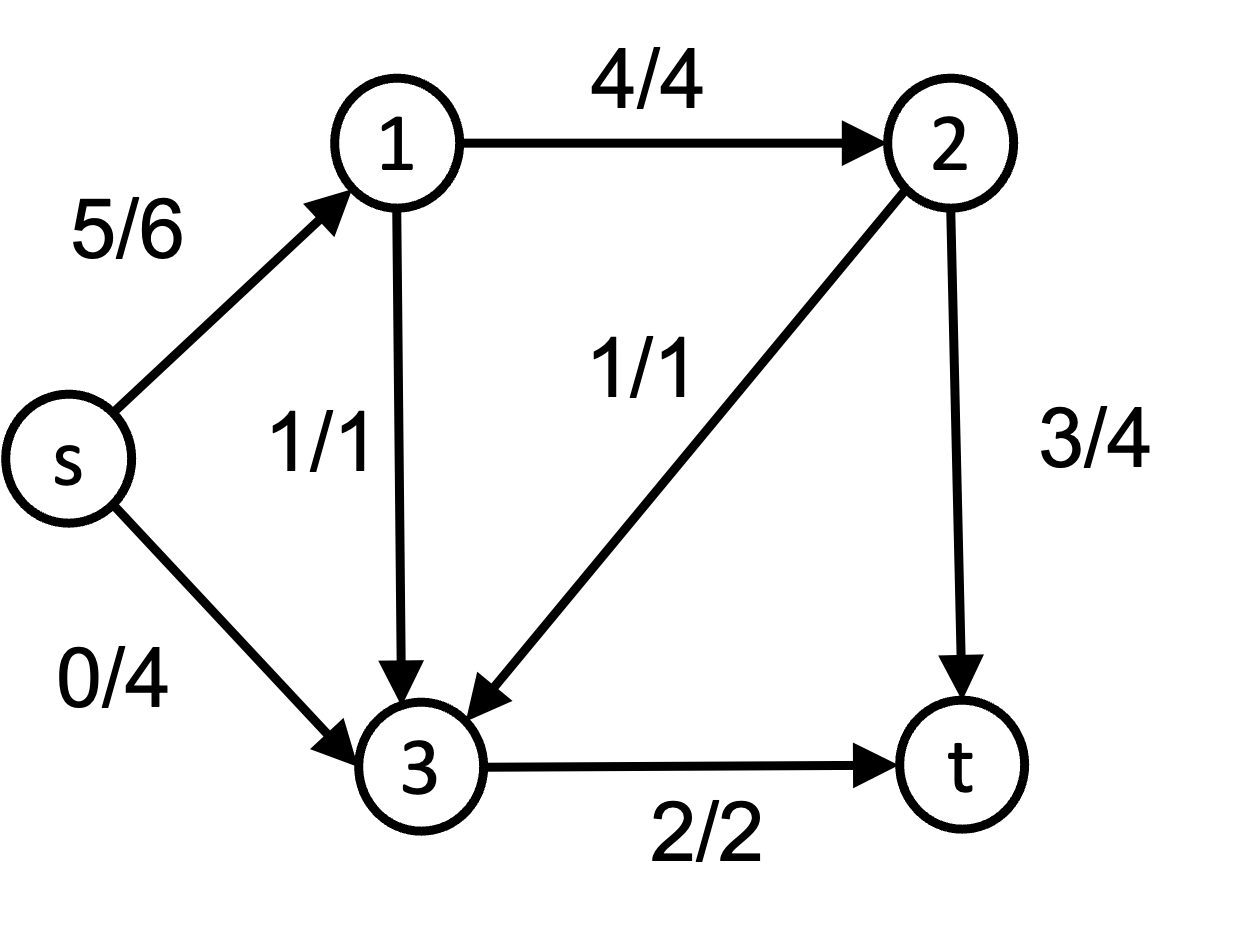
\includegraphics[width = .5\linewidth]{flow5.png} 
	
	\vs{2cm}
	
	
	
	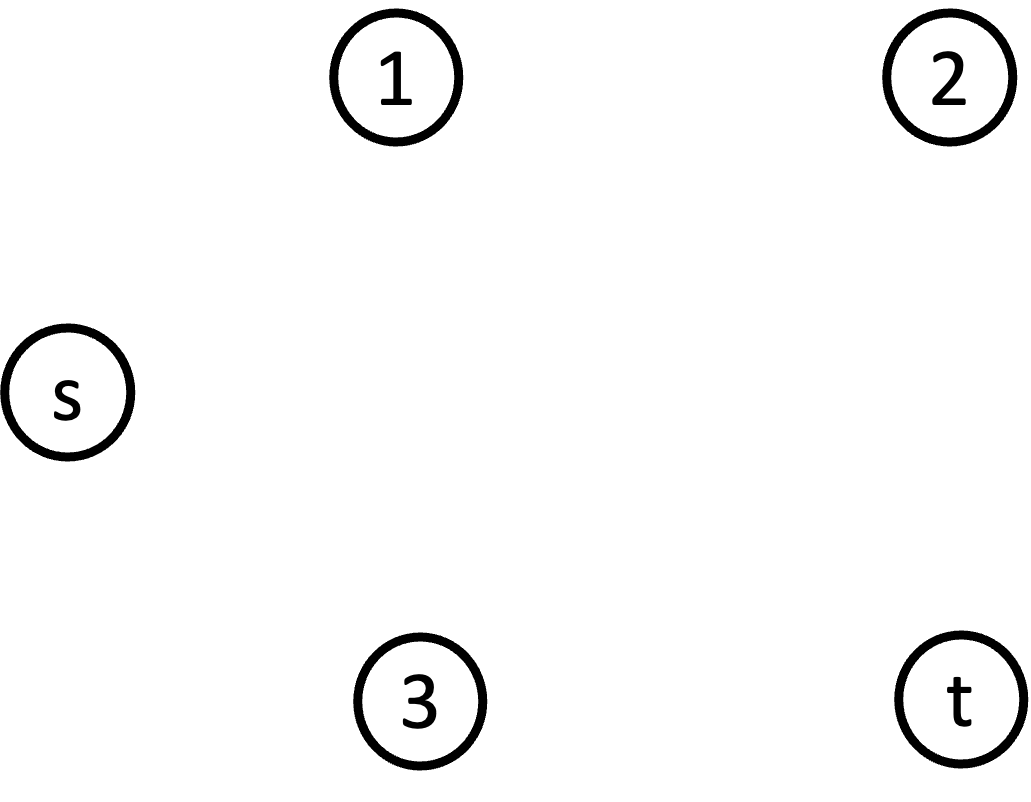
\includegraphics[width = .6\linewidth]{flow4empty.png} 
	
	
	\newpage
	
	\subsection{Augmenting Flows and Paths}
	Let $f$ be an $s$-$t$ flow in $G = (V,E)$ and $f'$ be a flow in the residual graph $G_f = (V,E_f)$. Then we define the \emph{augmentation} of $f$ by $f'$ as:
	
	\begin{equation}
		f \uparrow f' = f(u,v) + f'(u,v) - f'(v,u)
	\end{equation}
	
	\vs{.5cm}
	
	\begin{lemma}
		The function $f\uparrow f'$ is a valid flow in $G$, and it has flow value $|f| + |f'|$.
	\end{lemma}
	Proof: a whole bunch of bookkeeping. We will skip this. But we can illustrate it below.\\
	
	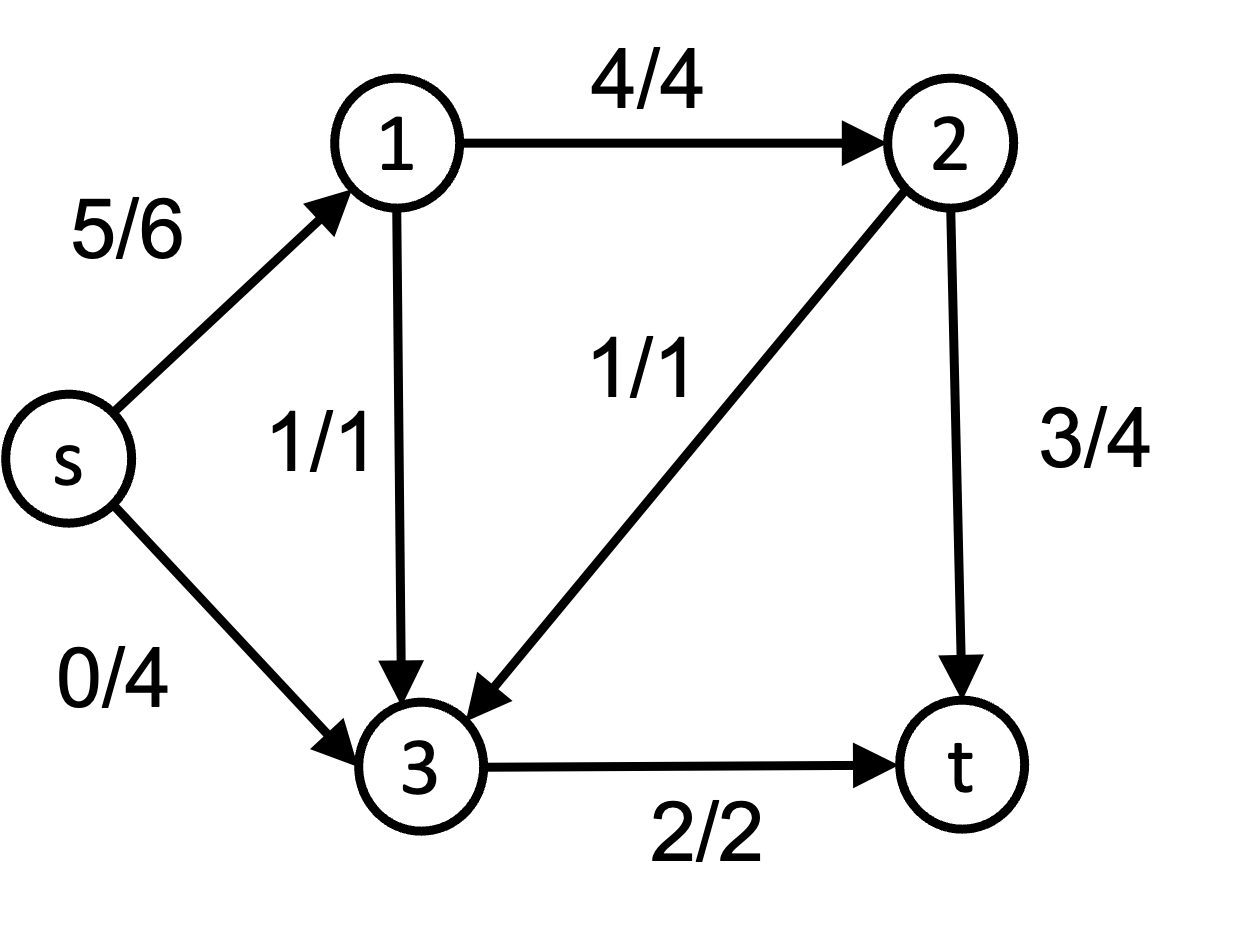
\includegraphics[width = .5\linewidth]{flow5.png} \hspace{1cm} 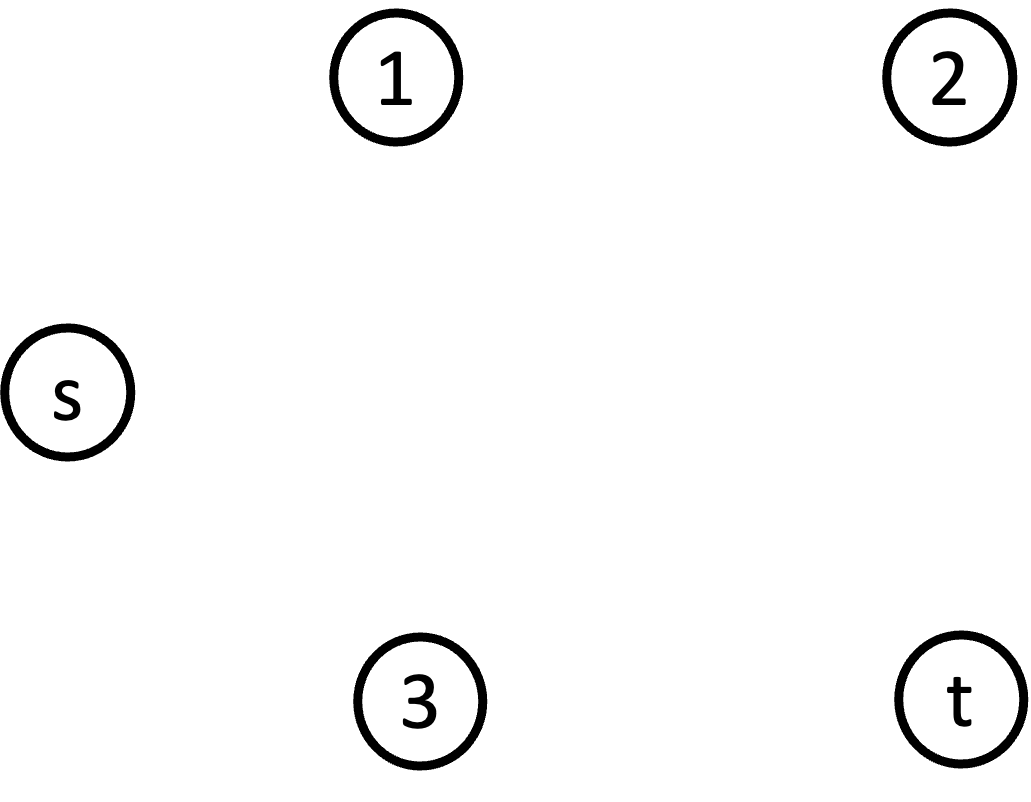
\includegraphics[width = .45\linewidth]{flow4empty.png} 
	
	\vspace{3cm} 
	
	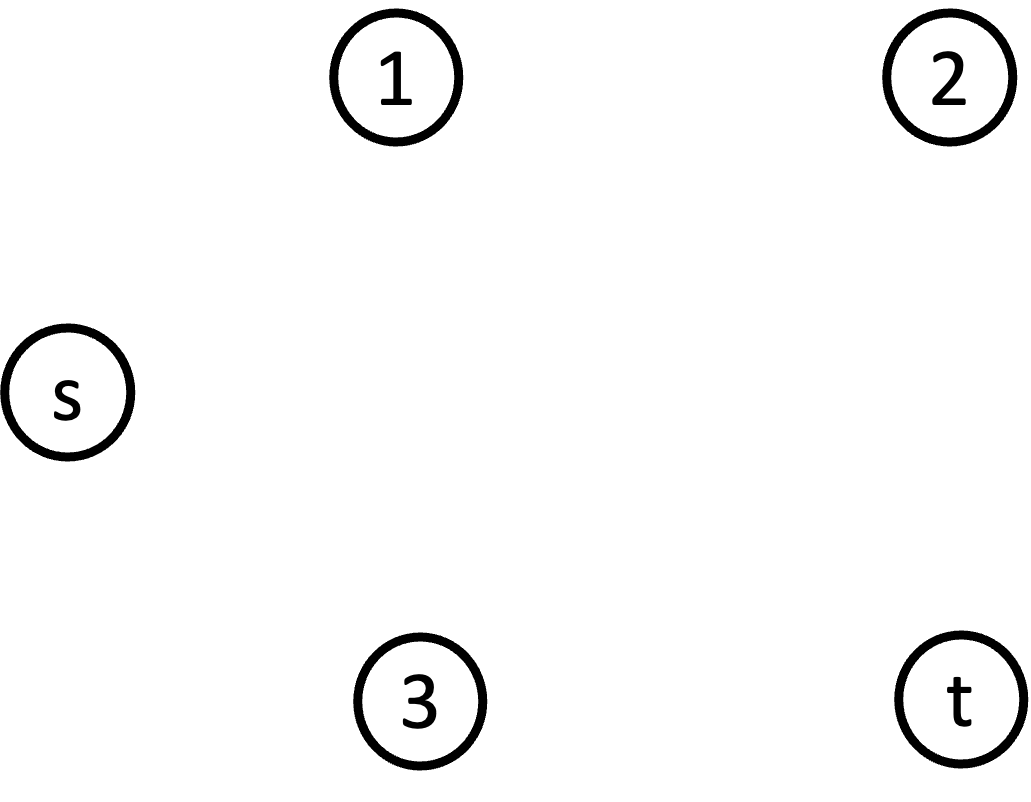
\includegraphics[width = .45\linewidth]{flow4empty.png} \hspace{2cm} 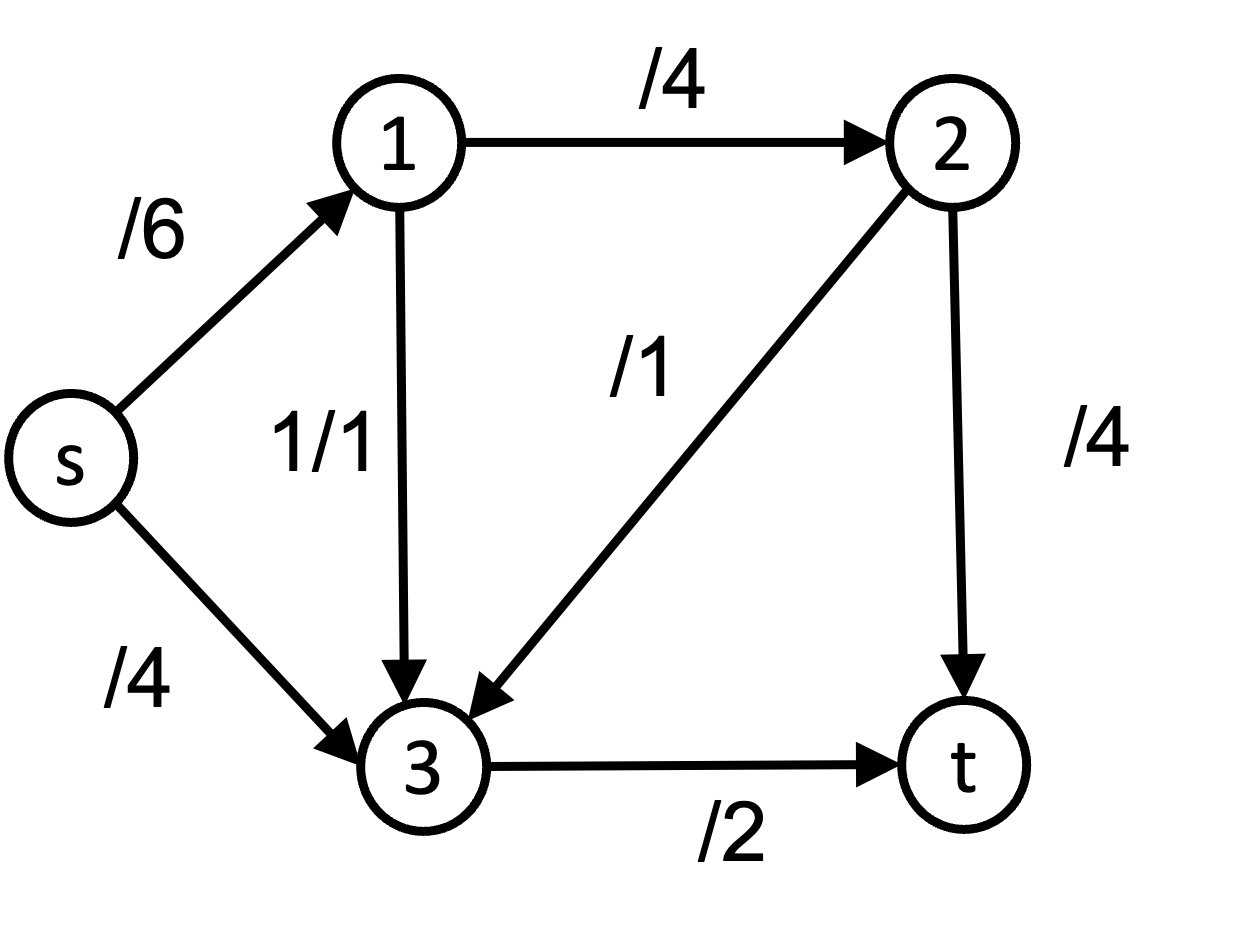
\includegraphics[width = .5\linewidth]{flow5noflow.png} 
	
	\newpage
	An \emph{augmenting path} $p$ is a simple path (simple = no cycles) from $s$ to $t$ in the residual network $G_f$.\\
	
	The \emph{residual capacity} of this path $p$ is the maximum amount we can send on $p$:
	
	%	$$c_f(p) = \min\{c_f(u,v) \colon (u,v) \text{ is in } p\}$$
	\vspace{2cm}
	
	Sending $c_f(p)$ flow along every edge in this path gives us a flow $f_p$ in $G_f$ that we can add to $f$ to improve it. \\
	
	
	\begin{theorem}
		(Max-flow Min-cut Theorem)
		Let $f$ be an $s$-$t$ flow on some graph $G = (V,E)$. The following three conditions are equivalent:
		\begin{enumerate}
			\item $f$ is a maximum $s$-$t$ flow
			\item There are no augmenting paths in the residual graph $G_f$
			\item %$|f| = \cut(S)$ for some $s$-$t$ cut set in $G$
		\end{enumerate}
	\end{theorem}
	
	\newpage
	\phantom{continued}
	
	
	\newpage
	\section{The Basic Ford-Fulkerson Algorithm}
	Idea: $f$ is a max-flow if and only if there are no augmenting paths. So let's just keep finding augmenting paths until we're done! \\
	
	The Ford-Fulkerson algorithm will always maintain the invariant that for any pair $(u,v)$, at most one of $\{f(u,v), f(v,u)\}$ will be greater than zero. \\
	
	\begin{algorithm}
		\textsc{FordFulkersonBasic}($G,s,t$)
		\begin{algorithmic}
			\For{$(u,v) \in E $}
			\State $f(u,v) = 0$
			\EndFor
			\While{there exists an $s$-$t$ path $p$ in $G_f$} 
			\State $c_f(p) = \min \{c_f(u,v) \colon (u,v) \text{ is in } p\}$
			\For{$(u,v) \in p$}
			
			\State $m = \min \{c_f(p), f(v,u)\}$ %\hfill // flow to ``undo''
			\State $\ell = c_f(p) - m$ %\hfill // new flow to send along $(u,v)$
			%		\If{$f(v,u) > 0$}	
			\State $f(v,u) \leftarrow f(v,u) - m$
			%		\EndIf
			\State $f(u,v) \leftarrow f(u,v) + \ell$
			%		\Else
			%		\State $f(v,u) \leftarrow f(v,u) - c_f(p)$
			%		\EndIf
			\EndFor
			\EndWhile
		\end{algorithmic}
	\end{algorithm}
	For $(u,v) \in p$, we first use any of the flow $c_f(p)$ to undo flow previously sent on $(v,u)$.\\
	
	Then, if any of $c_f(p)$ remains, we send it along $(u,v)$.
	
	\newpage
	\subsection{Runtime Analysis}
	\begin{itemize}
		\item $f^*$ is the maximum flow and $|f^*|$ the maximum flow value.
		\item Assume all weights are integers.
		\item Let $f$ be the flow we are growing as the algorithm progresses.
	\end{itemize}
	
	Answer the following questions:
	\begin{enumerate}
		\item What is the runtime complexity for finding an $s$-$t$ path $p$ in $G_f$?
		\item What is the minimum amount by which we can increase $f$ in each iteration?
		\item What is the maximum number of paths we might have to find before we are done?
		\item What is an overall runtime bound for \textsc{FordFulkersonBasic}?
	\end{enumerate}

\newpage

\subsection{How bad can the runtime be in practice?}

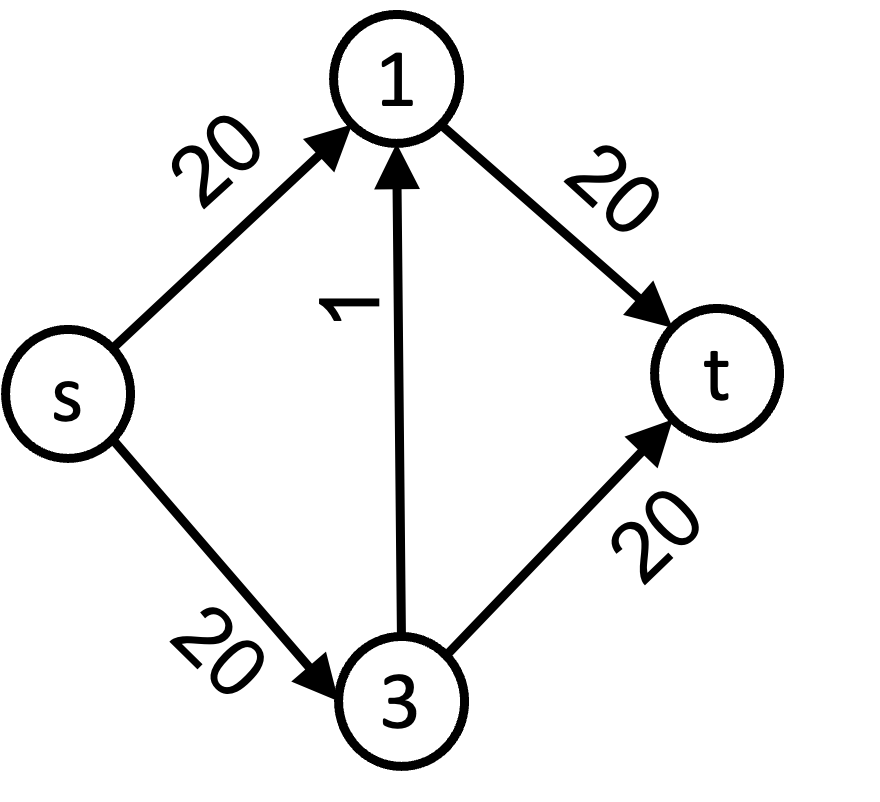
\includegraphics[width = .4\linewidth]{flow20pic.png} 

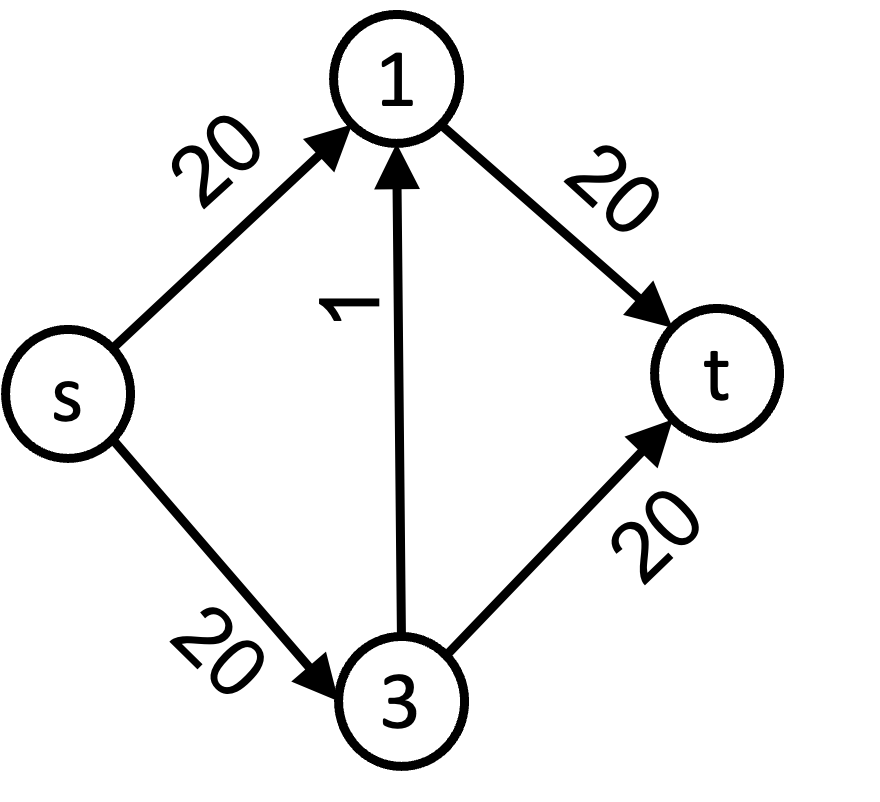
\includegraphics[width = .4\linewidth]{flow20pic.png} 

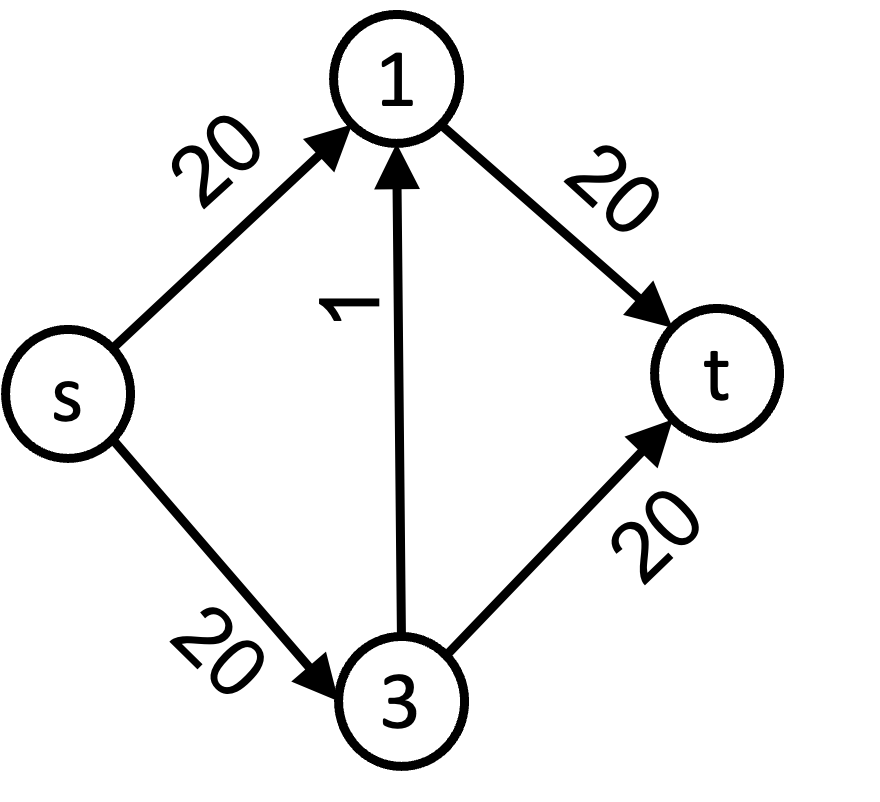
\includegraphics[width = .4\linewidth]{flow20pic.png} 

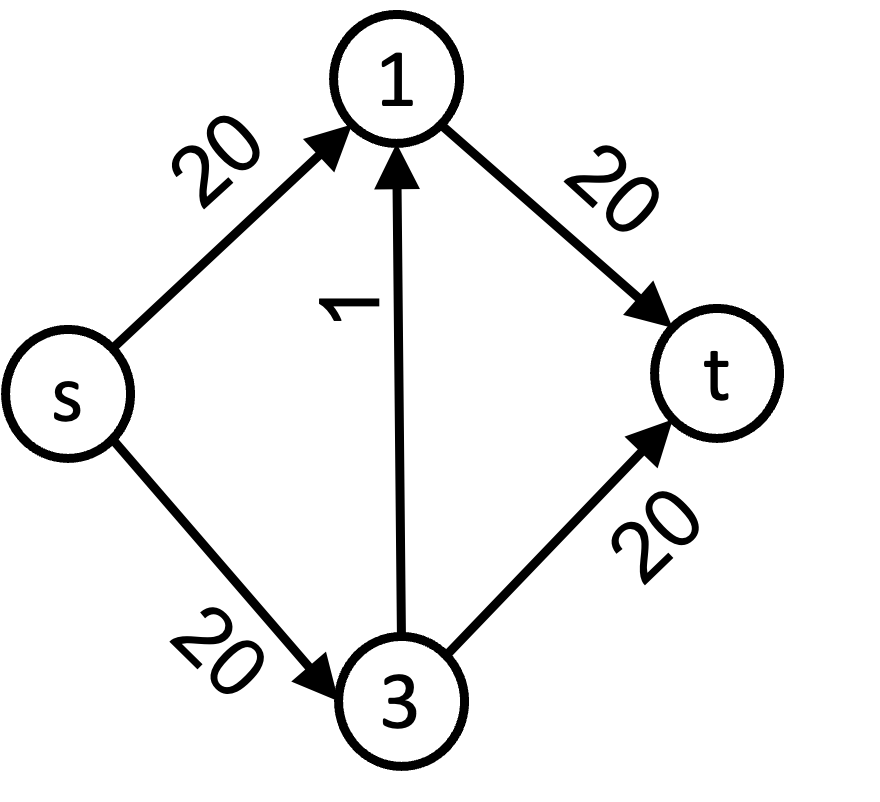
\includegraphics[width = .4\linewidth]{flow20pic.png} 

\newpage

\section{The Edmonds-Karp Algorithm}

The Edmonds-Karp Algorithm is a variation on Ford-Fulkerson that chooses an augmenting path $p$ by finding the directed path from $s$ to $t$ with the smallest number of edges.

\begin{Qu}
	Which algorithm should we use as a subroutine for finding paths for Edmonds-Karp?
	\begin{itemize}
		\aitem Breadth first search
		\bitem Depth first search
		\citem Topological sort
		\ditem Single source shortest path problem
		\eitem Hm...not sure.
	\end{itemize}
\end{Qu}

\subsection{Shortest path distances increases monotonically}

Let $f$ be an $s$-$t$ flow for input $G = (V,E,s,t)$ and $G_f$ be the residual graph. Define\\

\begin{equation*}
	\delta_f(s,v) = \text{ the shortest unweighted path distance from $s$ to $v$ in $G_f$}
\end{equation*}

\begin{lemma}
	For every $v \in V$, the distance $\delta_f(s,v)$ increases monotonically with each flow augmentation.\\
\end{lemma}

Translation: as we keep finding augmenting paths $p$ and sending more flow $f_p$ to $f$, the distance between $s$ and every node either stays the same, or increases. \\


\newpage

\begin{theorem}
	The total number of flow augmentation steps performed by Edmonds-Karp is $O(VE)$.
\end{theorem}

\begin{proof}
	
	
	\begin{itemize}
		\item Let $p$ be an augmenting path in $G_f$.\\
		
		\item An edge $(u,v) \in p$ is \emph{critical} if $c_f(p) = c_f(u,v)$, meaning it is the smallest capacity edge in that path. \\
		
		\item When we push $c_f(p)$ flow through $p$, the edge $(u,v)$ disappears from $G_f$
		
		\vs{2cm}
		
		%			\emph{It is either an edge $(u,v) \in E$ that gets completely saturated, or we are completely undoing all the flow on an edge $(v,u)$.} \\
		
		\item At least one edge on each path $p$ is critical.
		
		
		\item Claim: Each of the $|E|$ edges can be critical at most $|V|/2$ times.
		
		%			\textit{This would prove the result: there are $O(E)$ node pairs that can be an edge in $G_f$, and each of these can be critical at most $O(V)$ times, and since at least one edge is critical in each iteration, there can be at most $O(VE)$ iterations.} \\
	\end{itemize}
	\newpage
	\begin{itemize}
		
		\textbf{Proving the claim}: (u,v) becomes critical at most $|V|/2$ times.
		
		\item Let $u$ and $v$ be nodes in some edge in $E$. \\
		\item When $(u,v)$ is critical for the first time, $\delta_f(s,v) = \delta_f(s,u) + 1$ \\
		
		\textit{Because they are on a shortest path} \\
		
		\item Then $(u,v)$ disappears from the residual graph, and can only re-appear after $(v,u)$ is on some future augmenting path. Say that $(v,u)$ is on an augmenting path when the new flow on $G$ is $f'$, then 
		
		\begin{equation*}
			\delta_{f'}(s,u) = \delta_{f'}(s,v) + 1.
		\end{equation*}
		
		
		\item We know that $\delta_f(s,v) \leq \delta_{f'}(s,v)$ \\ %\emph{by the previous Lemma} \\
		
		\item So we have
		\begin{align*}
			\delta_{f'}(s,u) =  %\delta_{f'}(s,v) + 1 \geq \delta_f(s,v) = \delta_f(s,u) + 2.
		\end{align*}
		
		\item From the first to the second time $(u,v)$ becomes critical, the distance from $s$ to $u$ increases by at least 2.\\
		
		%		\item The distance from $s$ to $u$ is at most $|V|$.
		
		\item If $(u,v)$ becomes critical more than $|V|/2$ times, then the distance from $s$ to $u$ increases by more than $2 |V|/2 \geq |V|$.\\
		
		\vs{2cm}
		%			\emph{Contradiction: the distance from $u$ to $v$ is at most $|V|$.} \\
		
		\item Thus, $(u,v)$ becomes critical at most $|V|/2 = O(V)$ times.
	\end{itemize}
\end{proof}


\end{document}